\documentclass[12pt,a4paper]{report}
\usepackage[utf8]{inputenc}
\usepackage[top=2cm,bottom=1cm,right=1.5cm,left=1.5cm]{geometry}
\usepackage{amsmath,amsfonts,amssymb,mathrsfs,tikz,setspace}
\pagestyle{empty}
\setstretch{1.3}
\parindent=0mm
\usetikzlibrary{arrows,shapes,shadows.blur}
\begin{document}
\raisebox{-1.5cm}{\includegraphics[width=2.5cm,height=3cm]{example-image}}
\hfill
\begin{minipage}[c]{12cm}
\centering\bf
UNIVERSITE MOUHAMED BOUDIAF ..\\
Faculté des mathematiques et de l'informatique\\
Département de mathématiques
\end{minipage}
\hfill
\raisebox{-1.5cm}{\includegraphics[width=2.5cm,height=3cm]{example-image}}\\[5mm]
\centering
\bf {\LARGE
MEMOIRE DE FIN D'ETUDE}\rm\vskip5mm
\flushleft\leftskip=2cm
\large Présenté pour l'obtention du Dipl\^ome de \bf MASTER\rm\vskip5mm
\begin{description}\leftskip=3cm
\item[\bf Domaine :] Mathématiques et informatique
\item[\bf Filière :] Mathématiques
\item[\bf Option :] Mathématiques Discrètes
\end{description}
\leftskip=0mm
\centering \bf PAR\vskip5mm
\centering \bf Sujet\\[5mm]
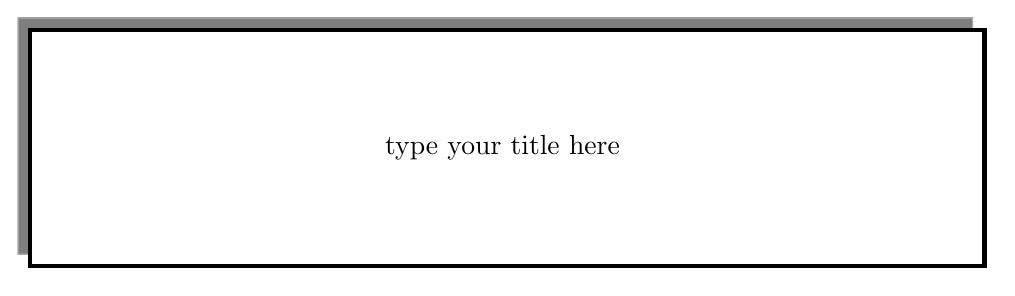
\begin{tikzpicture}
\node[fill=white,rectangle,draw,minimum width=\textwidth,minimum height=3cm,align=center,line width=1.5pt,blur shadow={shadow xshift=-1.5mm,shadow yshift=1.5mm,shadow scale=1,shadow blur radius=.1mm,shadow opacity=50}]{
type your title here
};
\end{tikzpicture}
\vskip5mm
\flushleft\bf Devant le jury:\rm\vskip3mm
\renewcommand{\arraystretch}{1.2}
\setlength{\tabcolsep}{8mm}
\begin{tabular}{lll}
text text text text&text&text\\
text&text&text\\
text&text&text\\
\end{tabular}
\vskip3cm
\centering
\bf Promotion : 2017/2018
\begin{tikzpicture}[remember picture,overlay]
\draw [line width=1.5pt]([shift={(1,1)}]current page.south west)rectangle([shift={(-1,-1)}]current page.north east);
\end{tikzpicture}
\end{document}